% ======================================================================
% BLOQUE 6 — HERON y cierre
% ======================================================================
\section{HERON y cierre}
\bloque{NEUTRINOS}

% ---------------------------------------------------------------- 50
\begin{frame}{El problema de la ultra alta energía: contar lo que casi no llega}
  \begin{columns}[c,onlytextwidth]
    \column{0.50\textwidth}
      \small
      \[ N_\nu = T\!\int\! dE\;\Phi_\nu(E)\,\big[A\Omega\big]_\mathrm{ef}(E) \]
      \vspace{-4pt}
      \begin{itemize}\footnotesize
        \item \textbf{Sección eficaz} $\sigma_{\nu N}(E)$: propiedad del neutrino.
        \item \textbf{Probabilidad de interacción} $P\simeq n\,\sigma\,L$ en un
          espesor $L$.
        \item \textbf{Volumen efectivo}: donde una interacción \emph{se detecta}.
        \item \textbf{Aceptación} $[A\Omega]_\mathrm{ef}$ (km$^2$\,sr) y
          \textbf{exposición} (km$^2$\,sr\,año): lo que el detector
          realmente integra.
      \end{itemize}
    \column{0.47\textwidth}
      \begin{clave}
        A EeV los flujos esperados son tan bajos que se necesitan
        \textbf{cientos de km$^3$} efectivos.
      \end{clave}
      \vspace{3pt}
      {\footnotesize
      \textbf{Óptico}: la luz se absorbe en $\sim$100\,m: sensores cada
      $\sim$100\,m. 1\,km$^3$ son 5160 sensores; 100\,km$^3$ serían cientos de
      miles.\\[3pt]
      \textbf{Radio}: atraviesa km de hielo y decenas de km de aire. Pocas
      antenas cubren volúmenes enormes, con umbral más alto.}\\[5pt]
      {\footnotesize\color{itedaGray} El régimen existe: KM3NeT detectó un
      neutrino de $\sim$220\,PeV (KM3-230213A, \textit{Nature} 2025).}
  \end{columns}
\end{frame}

% ---------------------------------------------------------------- 51
\bloque{}
\begin{frame}[plain]
  \fondo[0.25]{externas/ischigualasto_valle.jpg}
  \velo[0.9]{l}
  \begin{tikzpicture}[remember picture, overlay]
    \node[anchor=west, text=white, align=left, text width=10cm]
      at ([xshift=0.8cm, yshift=0.3cm]current page.west) {%
      {\small\color{itedaOrange}\bfseries EL PRÓXIMO GRAN OBSERVATORIO\\DE NEUTRINOS, EN ARGENTINA}\\[8pt]
      {\fontsize{44}{48}\selectfont\bfseries HERON}\\[6pt]
      {\normalsize Hybrid Elevated Radio Observatory for Neutrinos}\\[4pt]
      {\small San Juan: sierras que miran un valle}};
  \end{tikzpicture}
  \creditoblanco{Foto: Valle de la Luna (Ischigualasto), extremo norte de la Sierra de Valle Fértil, San Juan. Paulakindsvater, CC BY-SA 4.0 (Wikimedia Commons)}
\end{frame}

% ---------------------------------------------------------------- 52
\bloque{HERON}
\begin{frame}{Escuchar lluvias: dos mecanismos de emisión en radio}
  \begin{columns}[T,onlytextwidth]
    \column{0.49\textwidth}
      \centering
      {\small\bfseries En el aire: emisión geomagnética}\\[3pt]
      \begin{tikzpicture}[x=1cm,y=1cm]
        \draw[itedaTealDark, very thick, -{Stealth}] (0,2.4) -- (0,0.4)
          node[pos=0, left, font=\scriptsize] {eje};
        \fill[itedaOrange!30] (-1.6,0.3) .. controls (0,0.75) .. (1.6,0.3) --
          (1.6,0.15) .. controls (0,0.6) .. (-1.6,0.15) -- cycle;
        \node[font=\scriptsize, anchor=west] at (1.65,0.25) {frente};
        \draw[cmbRojo, thick, -{Stealth}] (0.2,0.5) -- (1.1,0.5) node[right, font=\scriptsize] {$e^+$};
        \draw[cmbAzul, thick, -{Stealth}] (-0.2,0.5) -- (-1.1,0.5) node[left, font=\scriptsize] {$e^-$};
        \draw[verdeRadio, thick, -{Stealth}] (-2.0,2.2) -- (-1.2,2.2) node[right, font=\scriptsize] {$\vec B_\oplus$};
        \foreach \r in {0.6,0.9,1.2}{\draw[violetaNu, thick] (2.1,1.6) ++(150:\r) arc (150:210:\r);}
        \node[font=\scriptsize, text=violetaNu, align=center] at (2.4,2.4) {pulso de\\$\sim$ns};
      \end{tikzpicture}\\[2pt]
      {\footnotesize La fuerza de Lorentz separa $e^\pm$: una \textbf{corriente
      transversal} variable irradia en 30--200\,MHz, en forma
      \textbf{coherente}: $P\propto E^2$.}
    \column{0.48\textwidth}
      \centering
      {\small\bfseries En medios densos: efecto Askaryan}\\[3pt]
      \begin{tikzpicture}[x=1cm,y=1cm]
        \fill[hielo!20, rounded corners=3pt] (-2.3,-0.2) rectangle (2.3,2.5);
        \draw[itedaTealDark, very thick, -{Stealth}] (-1.9,1.15) -- (1.9,1.15);
        \fill[cmbAzul!60] (0.4,1.15) ellipse (0.5 and 0.18);
        \node[font=\scriptsize, text=white] at (0.4,1.15) {$-$};
        \draw[violetaNu, thick] (0.4,1.15) -- ++(56:1.3);
        \draw[violetaNu, thick] (0.4,1.15) -- ++(-56:1.3);
        \draw[itedaGray] (1.0,1.15) arc (0:56:0.6);
        \node[font=\scriptsize] at (1.25,1.5) {$56^\circ$};
        \node[font=\scriptsize, anchor=north] at (0,-0.2) {cascada en el hielo};
      \end{tikzpicture}\\[2pt]
      {\footnotesize La cascada acumula $\sim$20\% de \textbf{carga negativa
      neta}: cono Cherenkov \textbf{coherente} en radio (RNO-G, IceCube-Gen2).}
  \end{columns}
  \vspace{2pt}
  \begin{clave}
    HERON usa la \textbf{emisión geomagnética} de lluvias de $\tau$ en el aire.
  \end{clave}
\end{frame}

% ---------------------------------------------------------------- 53
\begin{frame}{HERON: Hybrid Elevated Radio Observatory for Neutrinos}
  \centering
  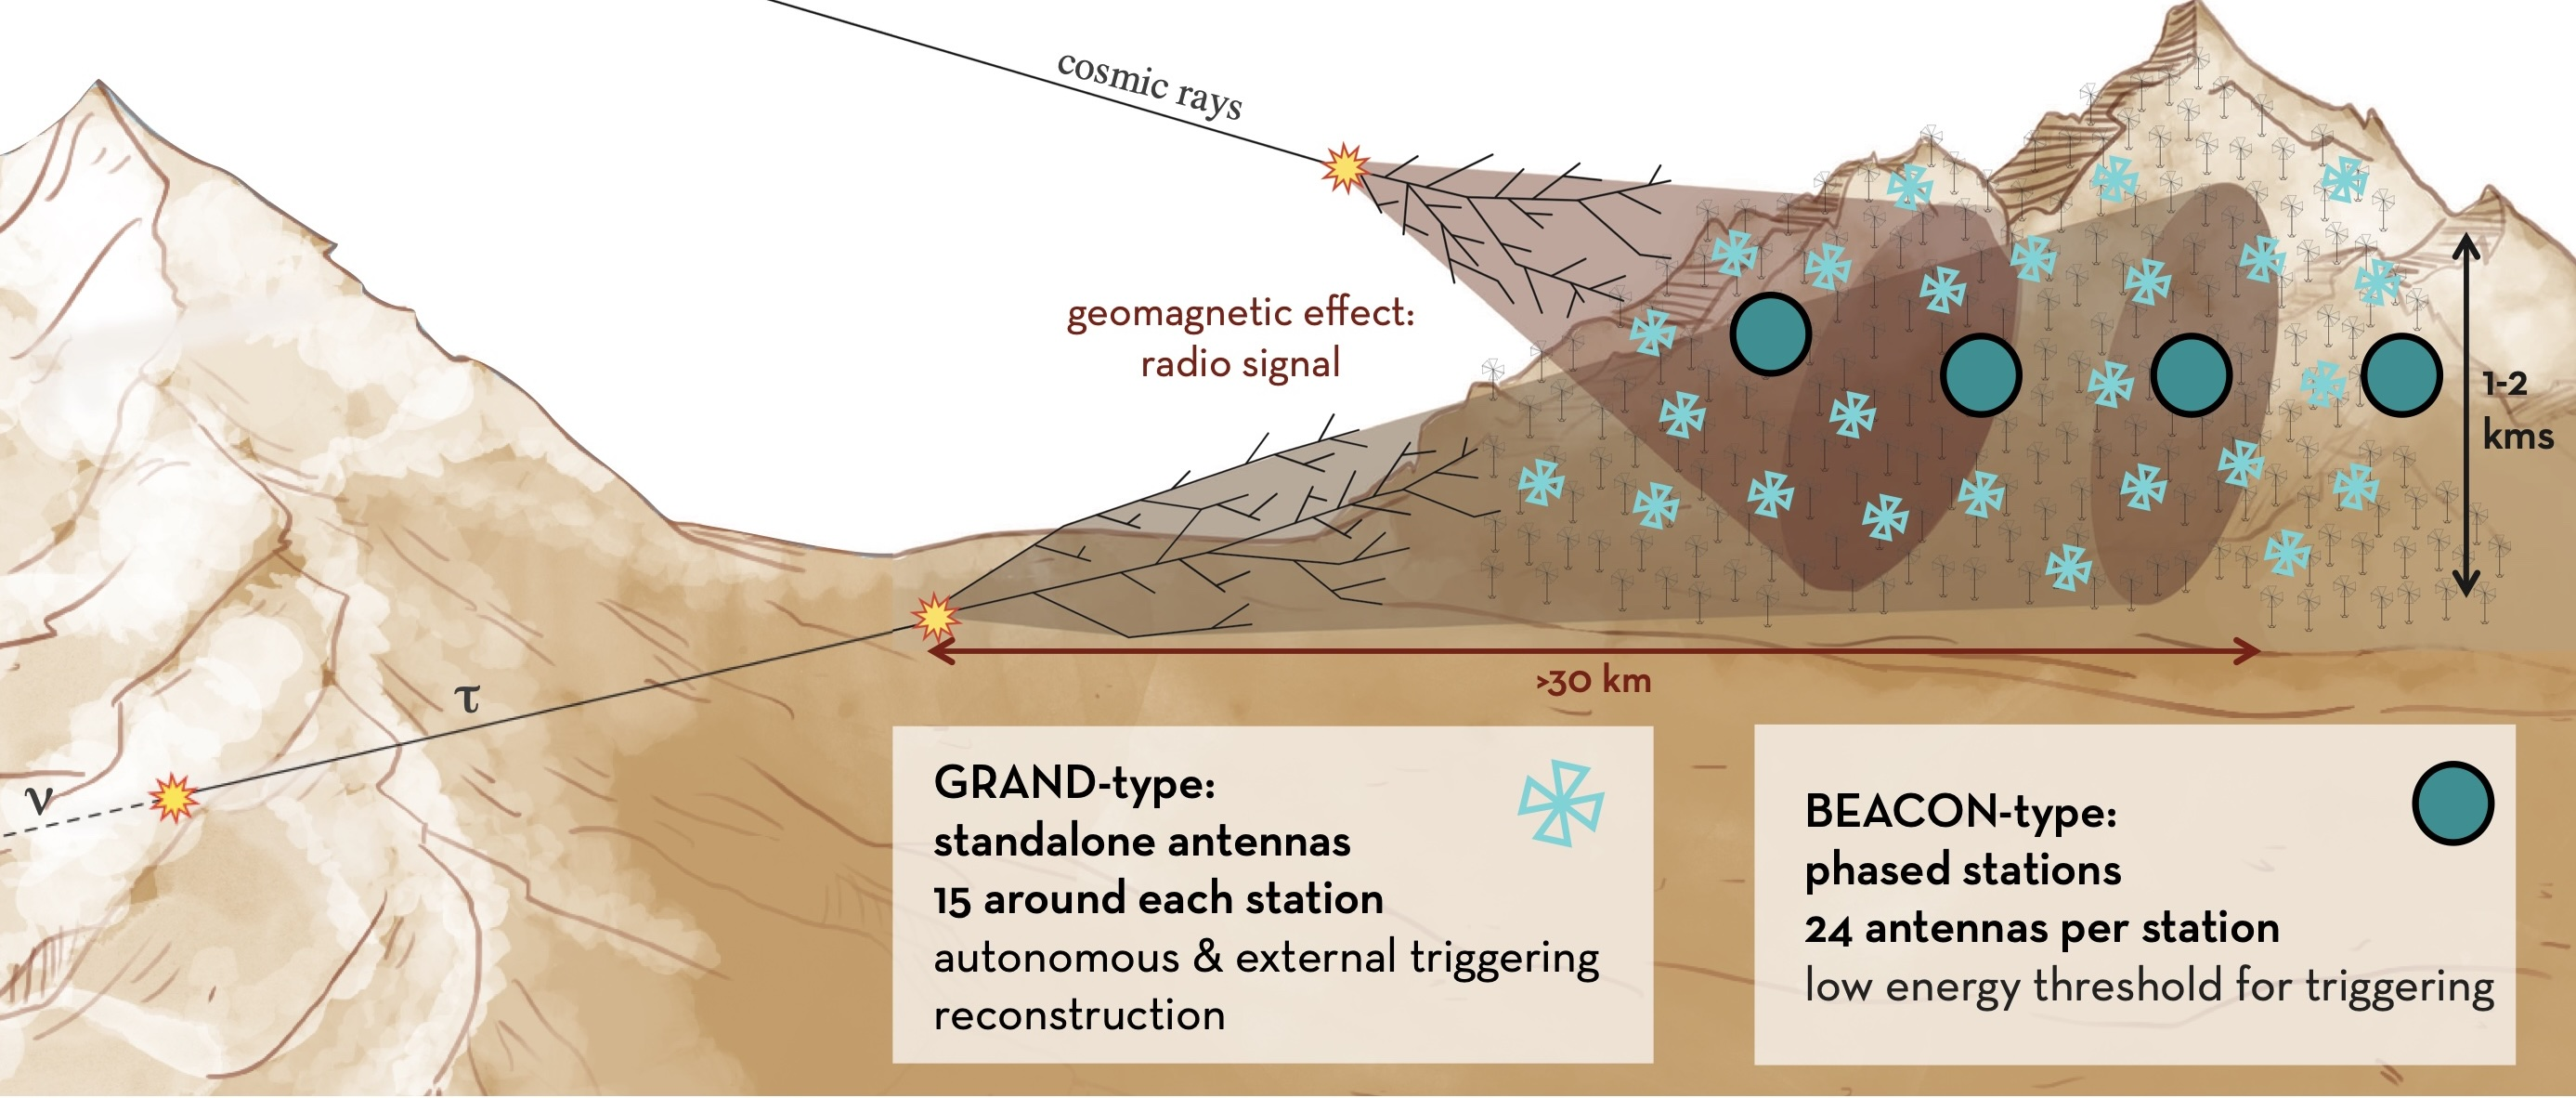
\includegraphics[width=0.66\linewidth]{heron/heron_concepto.png}\\[0pt]
  \begin{columns}[T,onlytextwidth]
    \column{0.50\textwidth}
      \footnotesize
      \begin{itemize}\footnotesize
        \item Un $\nu_\tau$ \textbf{roza la Tierra} y atraviesa la montaña:
          sale un $\tau$ que decae en el aire.
        \item Antenas en una ladera de \textbf{San Juan}, entre 1 y 2\,km sobre
          el valle.
      \end{itemize}
    \column{0.47\textwidth}
      \footnotesize
      \begin{itemize}\footnotesize
        \item \textbf{Híbrido}: 24 estaciones \emph{en fase} (BEACON) disparan;
          360 antenas autónomas (GRAND) reconstruyen.
        \item Objetivo: $\nu$ de $\sim$100\,PeV y \textbf{transitorios}.
      \end{itemize}
  \end{columns}
  \credito{Figura: K.~Kotera \textit{et al.} (BEACON y GRAND), PoS(ICRC2025), arXiv:2507.04382}
\end{frame}

% ---------------------------------------------------------------- 54
\begin{frame}{HERON desde San Juan}
  \begin{columns}[c,onlytextwidth]
    \column{0.36\textwidth}
      \centering
      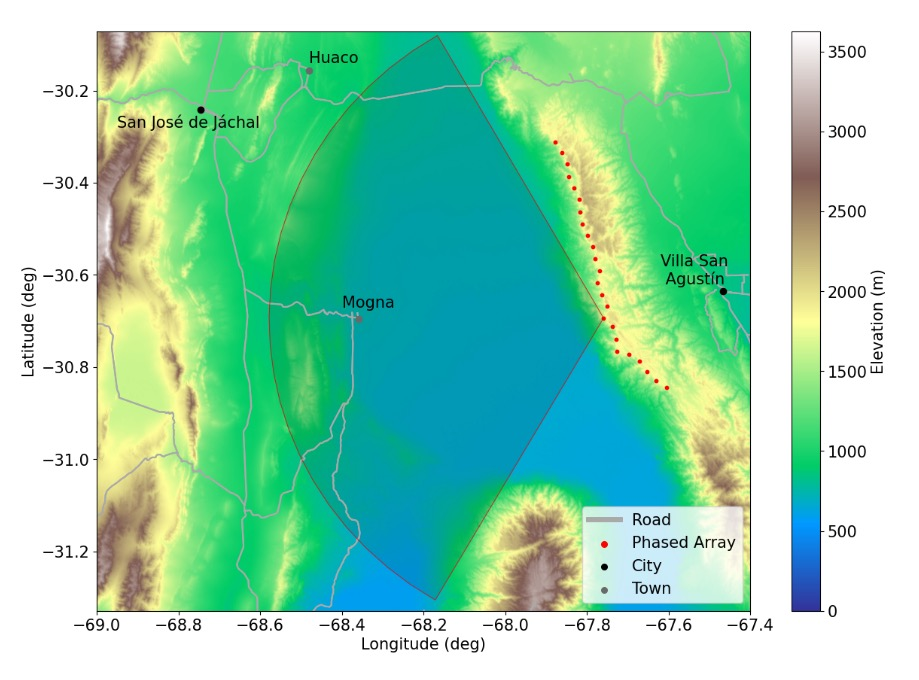
\includegraphics[width=0.84\linewidth]{heron/heron_sitio_mapa.png}\\[1pt]
      {\scriptsize 24 estaciones a lo largo de $\sim$70\,km de sierra, mirando
      un valle de 30--100\,km}
    \column{0.36\textwidth}
      \centering
      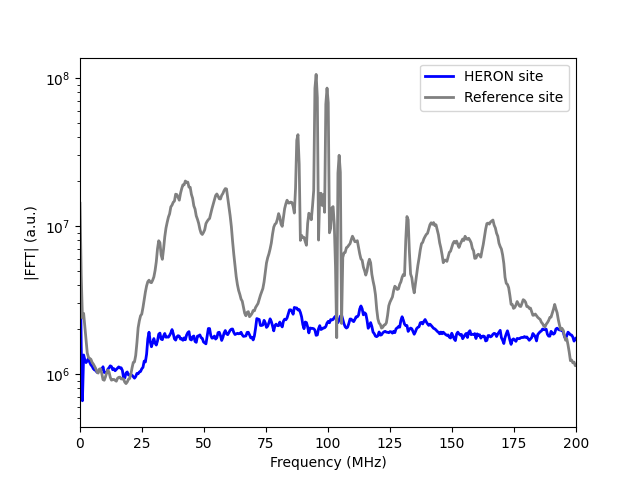
\includegraphics[width=0.88\linewidth]{heron/heron_ruido_sitio.png}\\[1pt]
      {\scriptsize Ruido de radio medido en el sitio (azul) frente a uno cerca
      de la ciudad (gris), abril de 2022}
    \column{0.25\textwidth}
      \begin{itemize}\scriptsize
        \item 936 antenas en total.
        \item Ve el 6\% del cielo a la vez y el 70\% por día.
        \item Proyecto de \textbf{I+D}, con diseño en optimización. Financiado
          por una \textbf{ERC Synergy Grant} y la ANR (Francia).
        \item CNEA (ITeDA, CAB), IAP--Sorbonne, IGFAE, Penn State.
      \end{itemize}
  \end{columns}
  \vspace{2pt}
  \begin{clave}
    No es un IceCube más grande: usa \textbf{la montaña como blanco} y
    \textbf{la atmósfera como calorímetro}.
  \end{clave}
  \creditoizq{Figuras: arXiv:2507.04382. Financiamiento y diseño: Zeolla, arXiv:2605.12081. Institucional: ITeDA}
\end{frame}

% ---------------------------------------------------------------- 55
\begin{frame}{HERON: cobertura del cielo y fuentes transitorias}
  \begin{columns}[c,onlytextwidth]
    \column{0.55\textwidth}
      \centering
      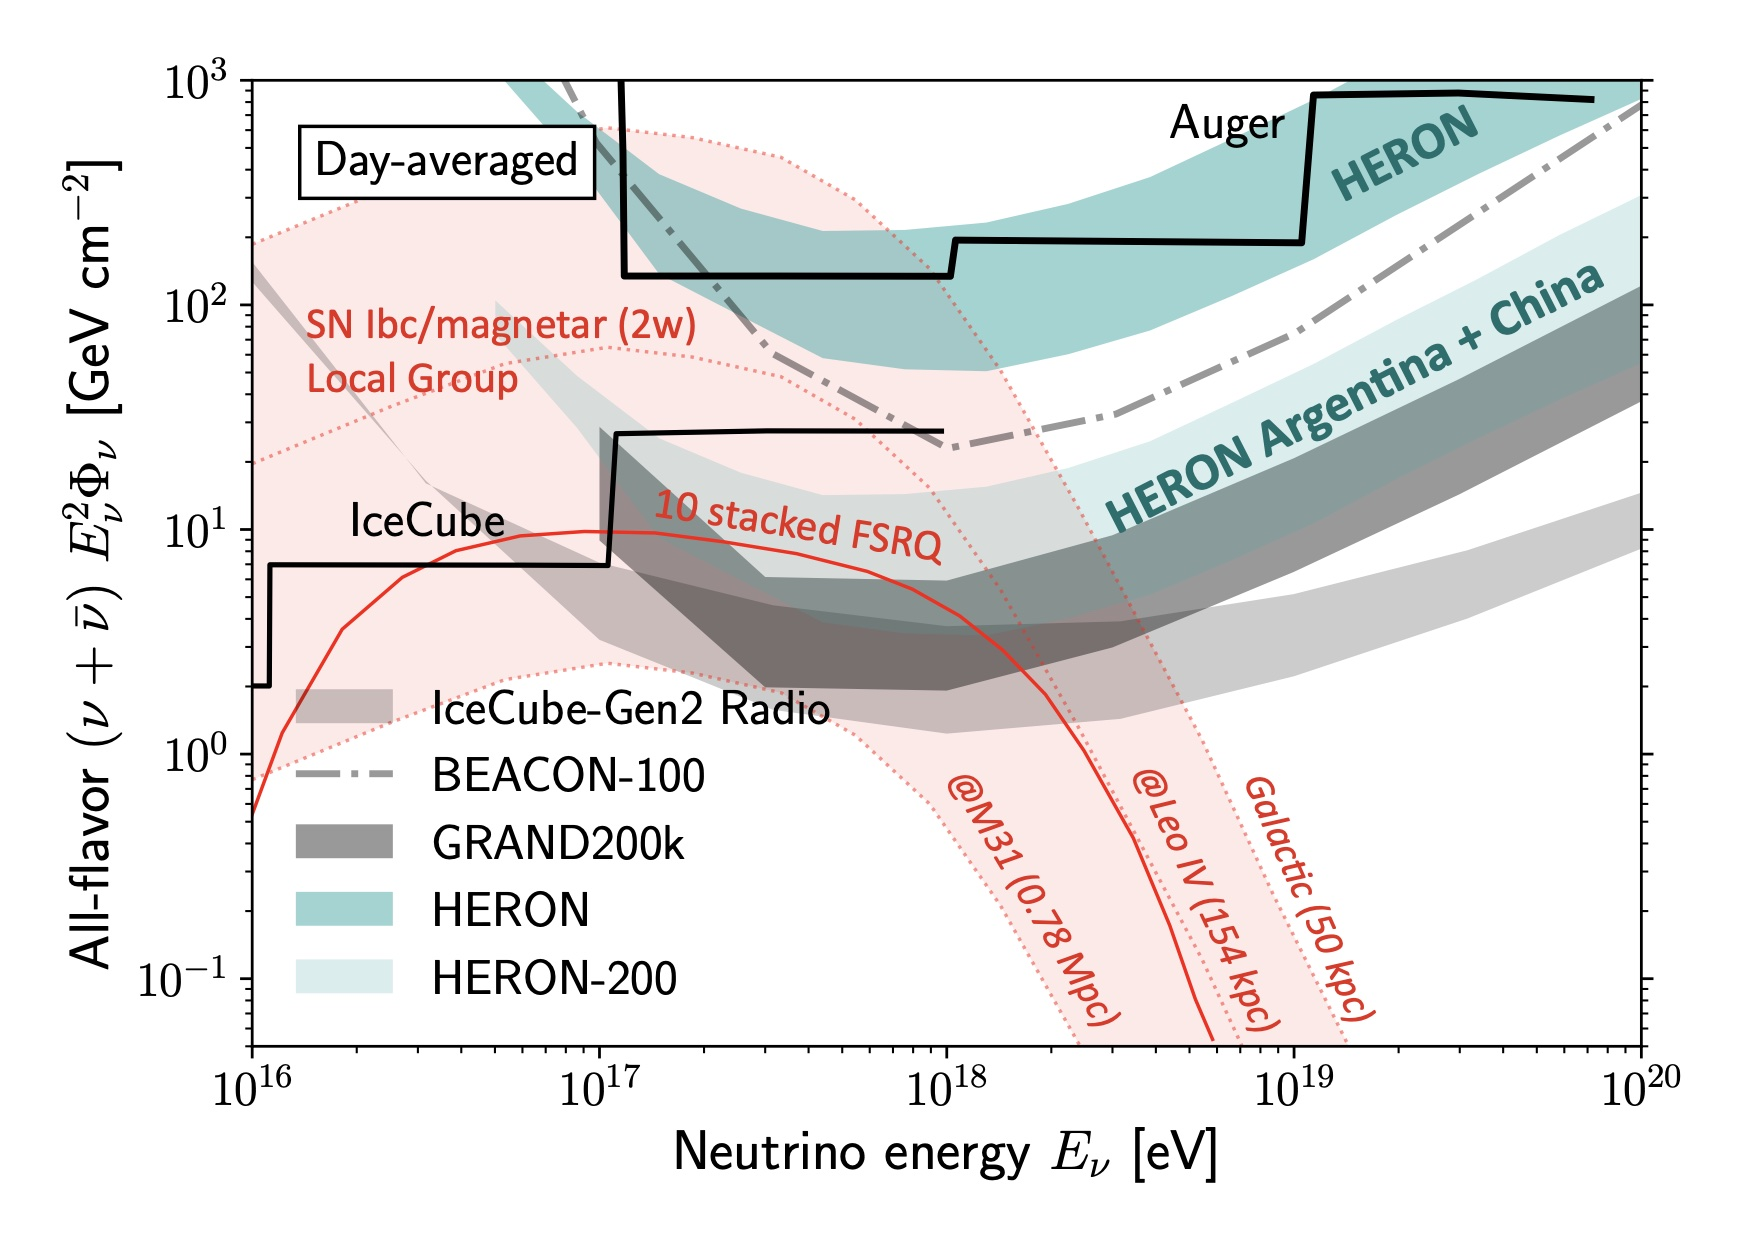
\includegraphics[width=\linewidth]{heron/heron_sensibilidad_dia.png}
    \column{0.42\textwidth}
      \small
      Sensibilidad promediada en un día, frente a IceCube, Auger y otros
      proyectos de radio (BEACON, GRAND, IceCube-Gen2 Radio).
      \begin{clave}
        HERON apunta a fuentes \textbf{transitorias} ---estallidos de rayos
        gamma, magnetares recién nacidos---, dentro de la red mundial de
        alertas multimensajero.
      \end{clave}
      {\footnotesize Para estallidos cortos, $\sim$10 veces mejor que los
      límites actuales de IceCube y Auger.}
  \end{columns}
  \credito{arXiv:2507.04382, Fig.~6; Zeolla, arXiv:2605.12081}
\end{frame}

% ---------------------------------------------------------------- 56
\begin{frame}{HERON frente a IceCube}
  \begin{columns}[c,onlytextwidth]
    \column{0.56\textwidth}
    \begin{tikzpicture}
      \begin{loglogaxis}[coloquio, width=\linewidth, height=6.1cm,
        xmin=1e15, xmax=1e20, ymin=1, ymax=2e7,
        xlabel={energía del neutrino [eV]}, ylabel={área efectiva [m$^2$]},
        xtick={1e15,1e16,1e17,1e18,1e19,1e20},
        ytick={1,1e2,1e4,1e6}, grid=major,
        legend style={at={(0.98,0.03)}, anchor=south east, font=\scriptsize,
          fill=white, fill opacity=0.9, text opacity=1, draw=itedaGray!40}]
        \fill[itedaOrange!14] (axis cs:5e16,1) rectangle (axis cs:2e17,2e7);
        \addplot[very thick, cmbAzul] table[x=E_eV, y expr=\thisrow{A_km2}*1e6] {data/icecube_aeff.dat};
        \addlegendentry{IceCube (todo el cielo)}
        \addplot[very thick, verdeRadio, dashed] table[x=E_eV, y expr=\thisrow{A_km2}*1e6] {data/heron_aeff_aprox.dat};
        \addlegendentry{HERON (en su franja del cielo)}
        \node[font=\scriptsize\bfseries, text=itedaOrange, anchor=north] at (axis cs:1e17,1.6e7) {$10^{17}$\,eV};
        \node[font=\scriptsize\bfseries, text=cmbAzul, fill=white, inner sep=1pt, anchor=north west]
          at (axis cs:1.3e17,700) {$\sim$1.000\,m$^2$};
        \node[font=\scriptsize\bfseries, text=verdeRadio, fill=white, inner sep=1pt, anchor=south east]
          at (axis cs:9e16,3e4) {$\sim$30.000\,m$^2$};
        \draw[-{Stealth}, itedaGray] (axis cs:2e15,300) -- (axis cs:5.5e15,170);
        \node[font=\tiny, text=itedaGray, anchor=south] at (axis cs:2e15,300) {Glashow};
      \end{loglogaxis}
    \end{tikzpicture}
    \column{0.41\textwidth}
      \tikzset{cab/.style={font=\scriptsize\bfseries, text=white, rounded corners=1.5pt,
        minimum width=2.3cm, minimum height=0.45cm}}
      \renewcommand{\arraystretch}{1.2}
      \vspace*{-6pt}
      {\tiny
      \begin{tabular}{@{}>{\raggedright\arraybackslash}p{0.95cm}>{\raggedright\arraybackslash}p{2.3cm}>{\raggedright\arraybackslash}p{2.3cm}@{}}
        & \tikz\node[cab, fill=cmbAzul]{IceCube}; & \tikz\node[cab, fill=verdeRadio]{HERON};\\
        \textbf{Tamaño} & 1\,km$^3$ de hielo, 5160 sensores & $\sim$70\,km de sierra, 936 antenas\\
        \textbf{Energías} & $10^{10}$--$10^{16}$\,eV & $>10^{16}$\,eV, óptimo $10^{17}$\,eV\\
        \textbf{Cielo} & todo, siempre & 6\% a la vez, 70\% por día\\
        \textbf{Área a $10^{17}$\,eV} & $\sim$1.000\,m$^2$ & $\sim$30.000\,m$^2$\\
        \textbf{Eventos} & $\sim$100 sobre 60\,TeV en 7,5 años; ninguno firme sobre 10\,PeV & meta: $\nu$ de $\sim$200 GRB en 5--10 años\\
      \end{tabular}}\\[4pt]
      \begin{clave}[fontupper=\footnotesize]
        IceCube domina hasta el PeV. A $10^{17}$--$10^{18}$\,eV, HERON ve
        10--100 veces más, pero sólo en una franja del cielo.
      \end{clave}
  \end{columns}
  \creditoizq{IceCube: data release EHE (arXiv:2507.07497), HESE 7,5 años. HERON: arXiv:2507.04382, Fig.~4, leída a ojo}
\end{frame}

% ---------------------------------------------------------------- 57
\begin{frame}{Una red mundial de telescopios de neutrinos}
  \begin{columns}[c,onlytextwidth]
    \column{0.55\textwidth}
      \centering
      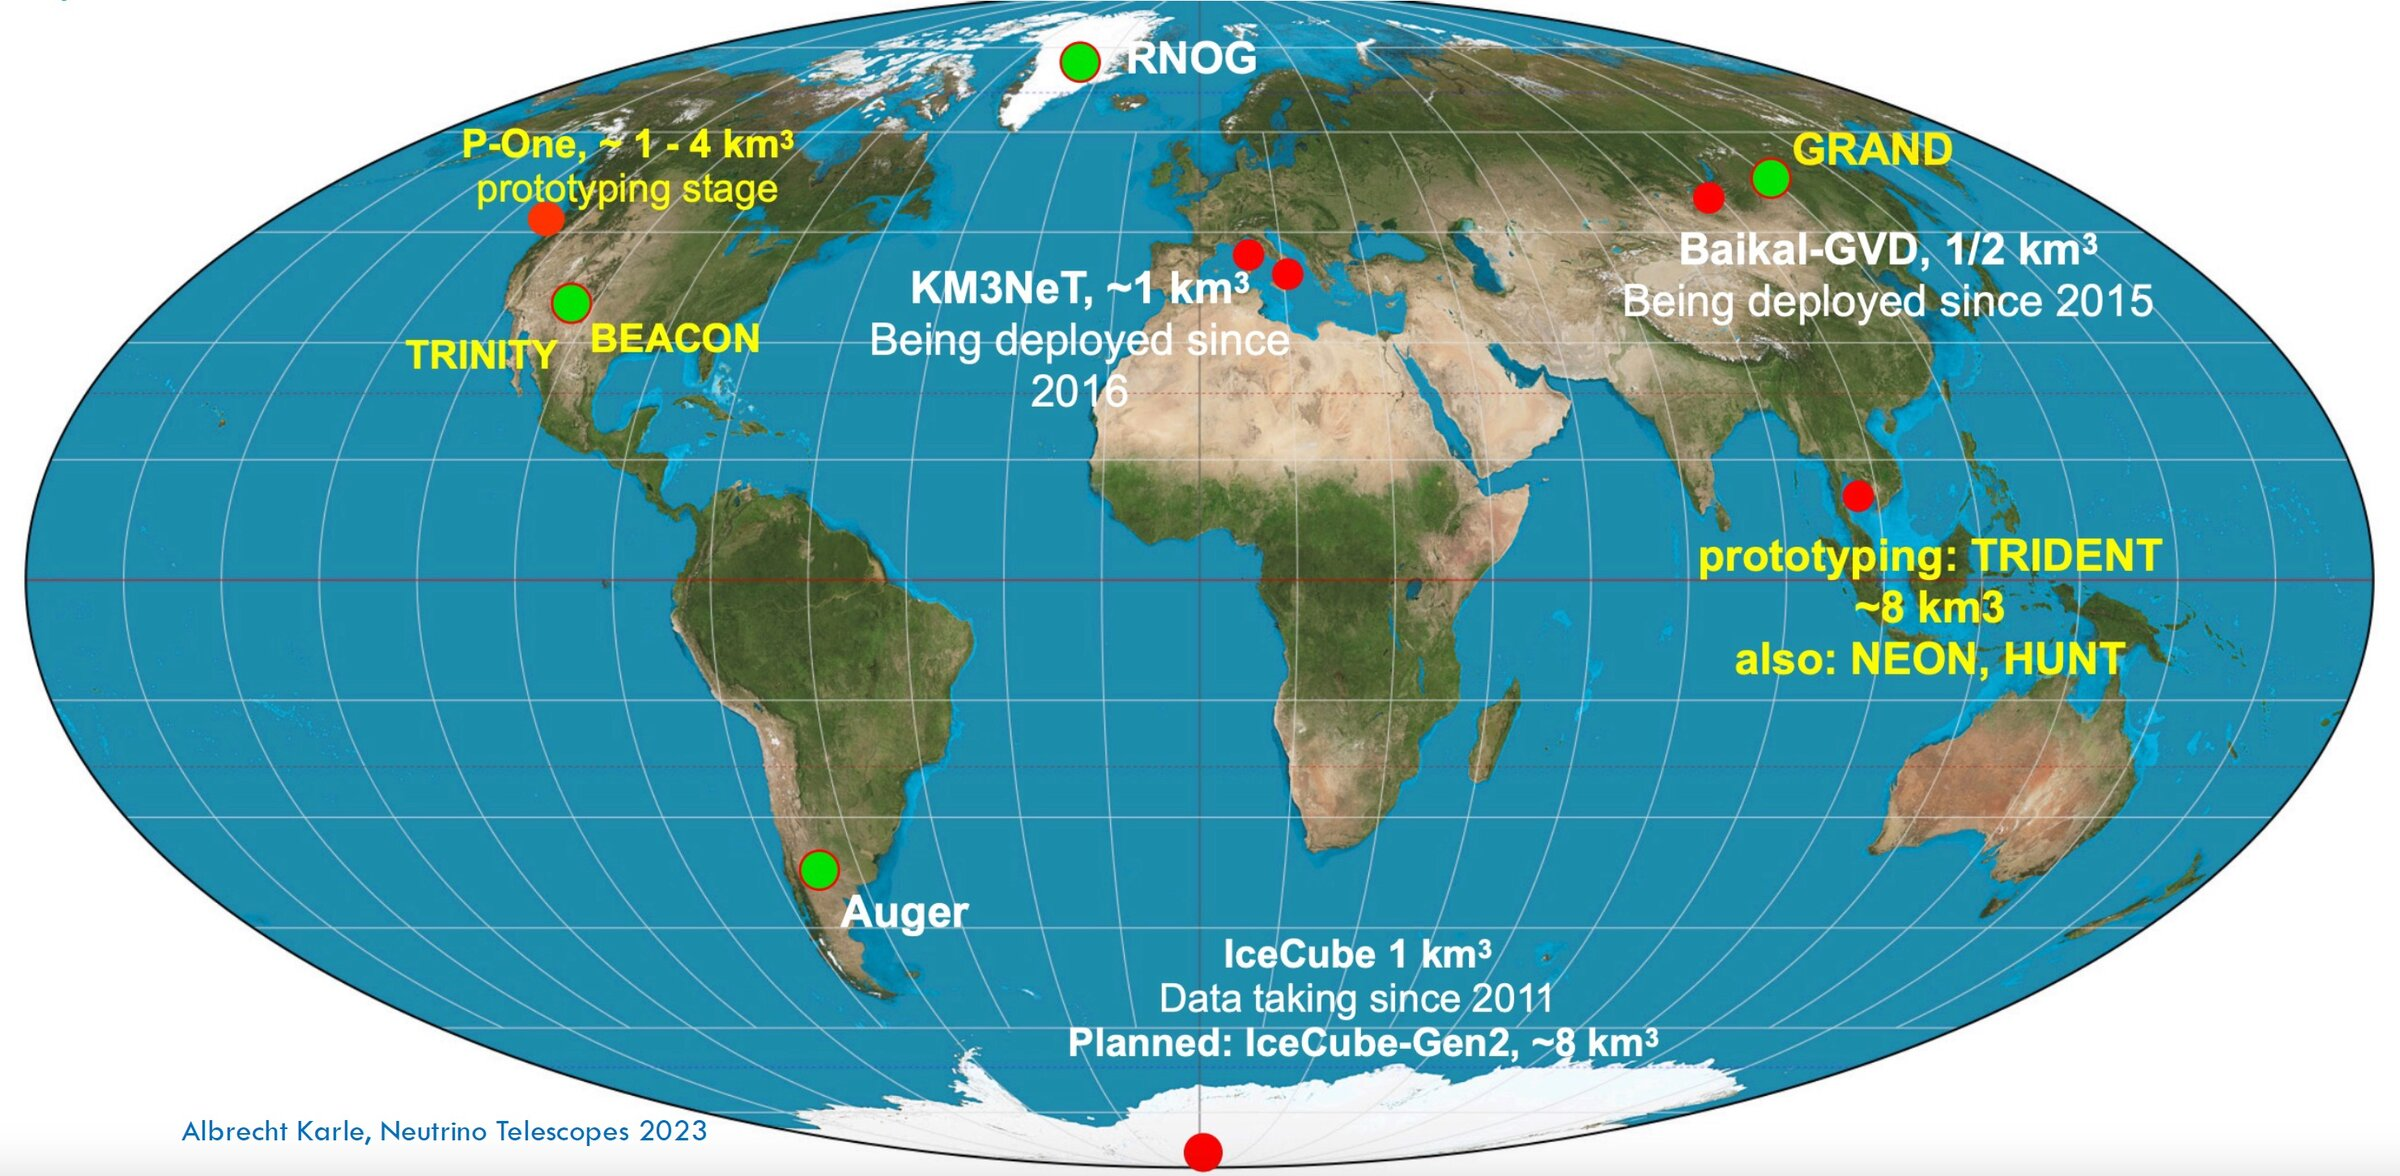
\includegraphics[width=\linewidth]{halzen/telescopios_neutrinos_mapa.jpg}
    \column{0.42\textwidth}
      \centering
      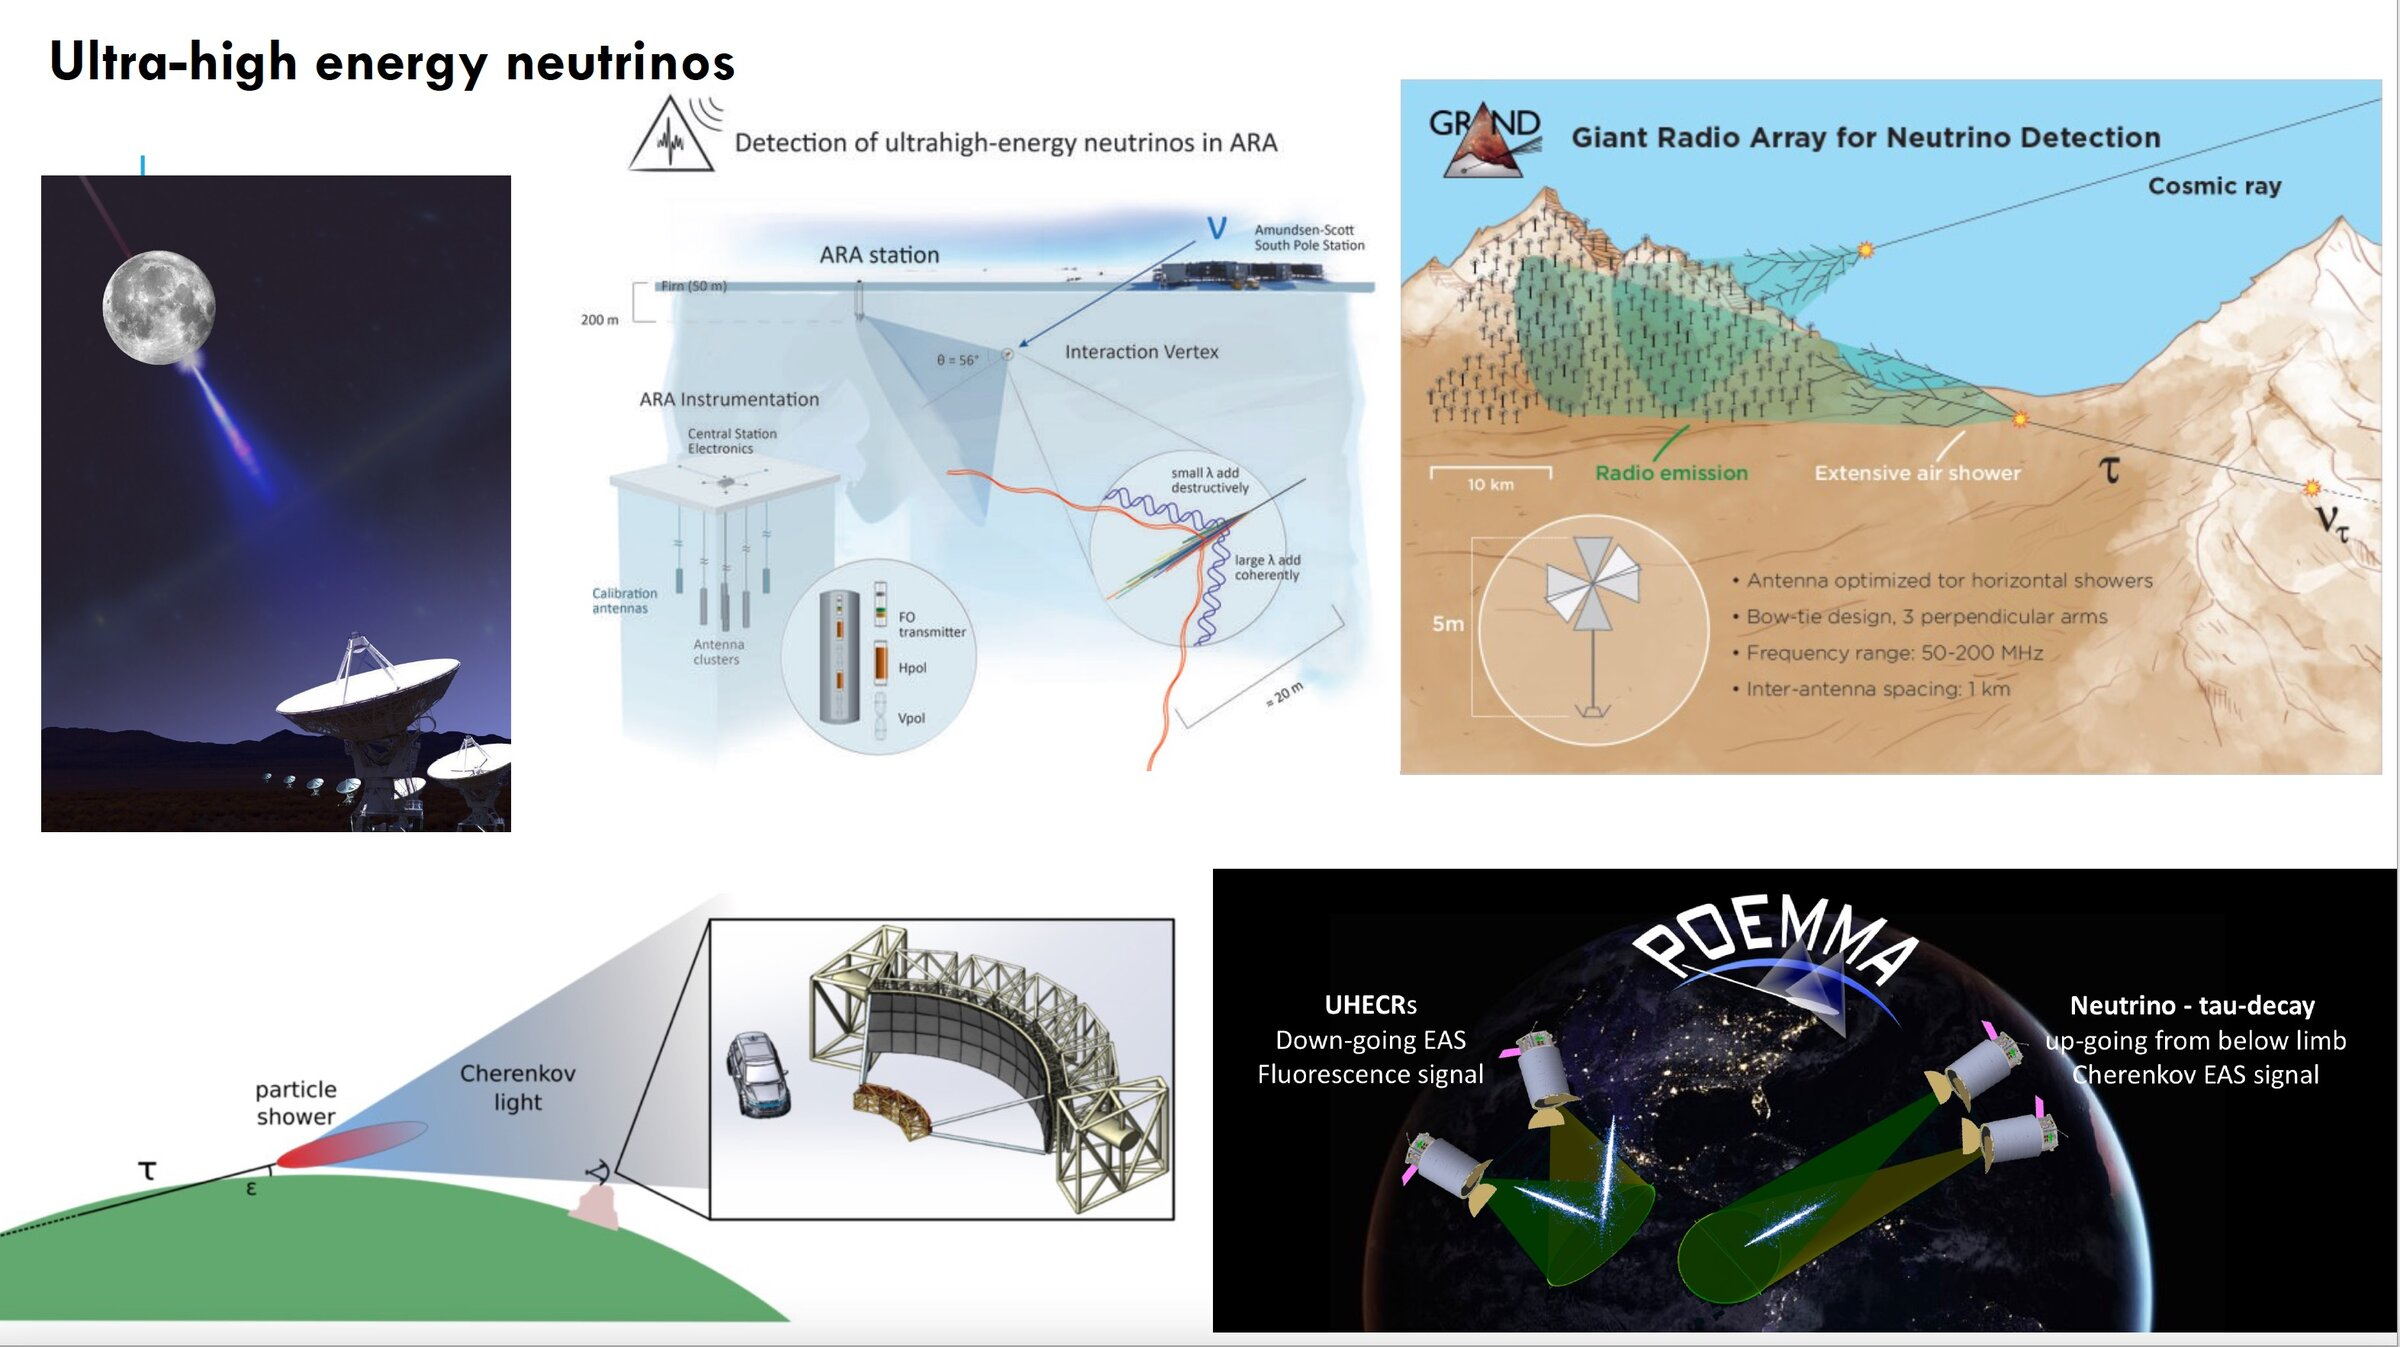
\includegraphics[width=\linewidth]{halzen/uhe_neutrinos_conceptos.jpg}\\[2pt]
      {\footnotesize Técnicas para ultra alta energía: radio en hielo, radio
      en el aire, lluvias de $\tau$ y observación desde el espacio. HERON
      suma a la Argentina a esa red.}
  \end{columns}
  \credito{Vía F.~Halzen (2024); mapa: A.~Karle, \textit{Neutrino Telescopes} 2022}
\end{frame}

% ---------------------------------------------------------------- 58
\bloque{CIERRE}
\begin{frame}{Tres soluciones experimentales a tres problemas físicos}
  \begin{tikzpicture}[x=1cm,y=1cm]
    \tikzset{
      cab/.style={font=\small\bfseries, text=white, minimum width=3.65cm,
        minimum height=0.6cm, rounded corners=2pt},
      celda/.style={font=\scriptsize, text width=3.5cm, align=left, anchor=north west},
      lab/.style={font=\scriptsize\bfseries, text=itedaGray, anchor=north east, align=right}}
    \node[cab, fill=itedaOrange] at (4.25,0) {Pierre Auger};
    \node[cab, fill=cmbAzul] at (8.1,0) {IceCube};
    \node[cab, fill=verdeRadio] at (11.95,0) {HERON};
    \foreach \y/\l/\a/\b/\c in {
        -0.5/{Mensajero}/{Rayos cósmicos}/{Neutrinos}/{$\nu_\tau$ que rozan la Tierra},
        -1.2/{Señal}/{Suelo, fluorescencia, radio}/{Luz Cherenkov en el hielo}/{Radio de lluvias en el aire},
        -1.9/{Geometría}/{Superficie de 3000\,km$^2$}/{Volumen de 1\,km$^3$}/{Ladera que mira un valle},
        -2.6/{Objetivo}/{Origen y composición de las partículas más energéticas}/{Dónde se aceleran los hadrones}/{$\nu$ de $\sim$100\,PeV y transitorios}}{
      \node[lab] at (2.3,\y) {\l};
      \node[celda] at (2.45,\y) {\a};
      \node[celda] at (6.3,\y) {\b};
      \node[celda] at (10.15,\y) {\c};
      \draw[itedaGray!30] (0.6,\y+0.08) -- (13.9,\y+0.08);}
    % eje de energía
    \begin{scope}[yshift=-4.75cm]
      \draw[itedaGray, thick, -{Stealth}] (2.3,0) -- (13.9,0);
      \foreach \e in {10,12,...,20}{
        \pgfmathsetmacro{\xx}{2.3+(\e-10)*1.05}
        \draw[itedaGray] (\xx,-0.07) -- (\xx,0.07) node[below=2pt, font=\tiny] {$10^{\e}$};}
      \node[lab, anchor=east] at (2.3,0.25) {Energía [eV]};
      \fill[cmbAzul, rounded corners=1pt] ({2.3+0*1.05},0.12) rectangle ({2.3+6*1.05},0.27);
      \node[font=\tiny\bfseries, text=cmbAzul, anchor=south] at ({2.3+3*1.05},0.27) {IceCube};
      \fill[itedaOrange, rounded corners=1pt] ({2.3+7*1.05},0.12) rectangle ({2.3+10.4*1.05},0.27);
      \node[font=\tiny\bfseries, text=itedaOrange, anchor=west] at ({2.3+10.45*1.05},0.2) {Auger};
      \fill[verdeRadio, rounded corners=1pt] ({2.3+6.7*1.05},0.36) rectangle ({2.3+9*1.05},0.51);
      \node[font=\tiny\bfseries, text=verdeRadio, anchor=east] at ({2.3+6.65*1.05},0.44) {HERON};
    \end{scope}
  \end{tikzpicture}
  \creditoizq{Rangos de energía aproximados}
\end{frame}

% ---------------------------------------------------------------- 59
\bloque{}
\begin{frame}[plain]
  \fondo[0.0][h]{tesis/auger_cr.jpg}
  \velo[0.75]{l}
  \begin{tikzpicture}[remember picture, overlay]
    \node[anchor=north west, text=white, align=left]
      at ([xshift=0.9cm, yshift=-0.9cm]current page.north west) {%
      {\fontsize{34}{38}\selectfont\bfseries ¡Gracias!}\\[6pt]
      {\Large\color{itedaOrange}\bfseries ¿Preguntas?}};
    \node[anchor=south west, text=white, align=left]
      at ([xshift=0.9cm, yshift=0.9cm]current page.south west) {%
      {\small Lautaro Silva Pizzi · ITeDA (CNEA--CONICET--UNSAM)}\\[2pt]
      {\small lautarosilvapizzi@gmail.com}};
    \node[anchor=south east, fill=white, rounded corners=2pt, inner sep=3pt]
      at ([xshift=-0.6cm, yshift=0.9cm]current page.south east)
      {
\includegraphics[height=0.95cm]{logos/logo-portada5-iteda.png}};
  \end{tikzpicture}
  \creditoblanco{Imagen: A.~Chantelauze, S.~Staffi, L.~Bret (Observatorio Pierre Auger)}
\end{frame}
